%%%%%%%%%%%%%%%%%%%%%%%%%%%%%%%%%%%%%%%%%%%%%%%%%%%%%%%%%%%%%%%%
%
% Copyright (C) 2017-2019 Tactical Computing Laboratories, LLC
% All Rights Reserved
% contact@tactcomplabs.com
%
%%%%%%%%%%%%%%%%%%%%%%%%%%%%%%%%%%%%%%%%%%%%%%%%%%%%%%%%%%%%%%%%

%----------------------------------------------------------------------------------------
%	PACKAGES AND DOCUMENT CONFIGURATIONS
%----------------------------------------------------------------------------------------

\documentclass{article}

\usepackage[margin=1.0in]{geometry}
\usepackage[version=3]{mhchem} % Package for chemical equation typesetting
\usepackage{siunitx} % Provides the \SI{}{} and \si{} command for typesetting SI units
\usepackage{graphicx} % Required for the inclusion of images
%\usepackage{natbib} % Required to change bibliography style to APA
\usepackage{amsmath} % Required for some math elements 
\usepackage[utf8]{inputenc}
\usepackage[english]{babel}
\usepackage[parfill]{parskip}
\usepackage{array}
\usepackage{algorithm}
\usepackage{algcompatible}
\usepackage{listings}
\usepackage{xcolor}
\usepackage{courier} % for \texttt{}
\usepackage{dirtree}
\usepackage{multirow}
%\usepackage{draftwatermark} % required for watermarks
\usepackage{vhistory}
\RequirePackage{epstopdf}
\RequirePackage{tabularx}
\RequirePackage{xstring}
\RequirePackage{hyperref}
\RequirePackage{fancyhdr}

%-- setup paragraphs and margins
\setlength{\parindent}{1em}
\setlength{\parskip}{1em}

%\SetWatermarkText{DRAFT}
%\SetWatermarkScale{5}

%-- code listing setup
\lstdefinestyle{base}{
  language=C++,
  numbers=left,
  stepnumber=1,
  emptylines=1,
  breaklines=true,
  basicstyle=\ttfamily\color{black},
  moredelim=**[is][\color{red}]{@}{@},
}

%-- setup hyperlinks
\hypersetup{
  colorlinks=true,
  linktoc=all,
  linkcolor=black,
  citecolor=black,
  urlcolor=black
}
%--

\setlength\parindent{0pt} % Removes all indentation from paragraphs

\renewcommand{\labelenumi}{\alph{enumi}.} % Make numbering in the enumerate environment by letter rather than number (e.g. section 6)

%\usepackage{times} % Uncomment to use the Times New Roman font
%----------------------------------------------------------------------------------------
%	DOCUMENT LAYOUT INFORMATION
%----------------------------------------------------------------------------------------
\pagestyle{fancy}
\lhead{}
\chead{\textbf{CoreGen IR Spec v.1.4.4}}
\rhead{}
\lfoot{} %-- format: TR YYYY-RRR-V.V; y = year; r = report; v = version
\cfoot{\textbf{CoreGen IR Spec v.1.4.4}}
\rfoot{\thepage}      % -- page number

%----------------------------------------------------------------------------------------
%	DOCUMENT INFORMATION
%----------------------------------------------------------------------------------------

\title{CoreGen Intermediate Representation\\Language Specification} % Title

\author{Tactical Computing Laboratories, LLC} % Author name

\date{} % Date for the report

\begin{document}

%-- begin TCL logo
\begin{figure}
\begin{center}

\includegraphics[width=3in]{figures/coregen-logo.png} % Include the logo
\end{center}
\end{figure}
%-- end TCL logo

\maketitle % Insert the title, author and date
\thispagestyle{fancy} %-- force the fancyhdr

\begin{center}
\begin{tabular}{l r}
Date: & August 27, 2019 \\ % Date the experiment was performed
Revision: & 1.4.4 \\         % revision number
Authors: & Tactical Computing Labs\\ % Author names
& contact@tactcomplabs.com\\
\end{tabular}
\end{center}

%----------------------------------------------------------------------------------------
%       TOC
%----------------------------------------------------------------------------------------

\clearpage
\tableofcontents
\clearpage

%----------------------------------------------------------------------------------------
%       List of Document Elements
%----------------------------------------------------------------------------------------

\clearpage
\listoffigures
\lstlistoflistings
\listoftables
%\listofalgorithms
\clearpage

%----------------------------------------------------------------------------------------
%       Changelog
%----------------------------------------------------------------------------------------

\clearpage
\begin{versionhistory}
  \vhEntry{1.0}{09.12.2018}{JLeidel}{Initial public release}
  \vhEntry{1.1}{11.21.2018}{JLeidel}{Adding ThreadUnits to Core nodes and TUSReg register attributes}
  \vhEntry{1.2}{11.21.2018}{JLeidel}{Adding subregister pseduoregister sub-node structure for setting up register aliases to specific bit regions of parent registers}
  \vhEntry{1.3}{12.20.2018}{JLeidel}{Adding clarifying text to indicate the permissible characters utilized in IR node names}
  \vhEntry{1.4}{01.21.2019}{JLeidel}{Adding RTL Type fields for overloaded RTL models; Adding Syntax mnemonic fields for instructions}
  \vhEntry{1.4.1}{04.24.2019}{JLeidel}{Adding PC attribute to register node attributes}
  \vhEntry{1.4.2}{07.03.2019}{JLeidel}{Adding Override keyword to all candidate hardware nodes: Section 2.3}
  \vhEntry{1.4.3}{08.21.2019}{JLeidel}{Adding syntax mnemonics to pseudo instructions}
  \vhEntry{1.4.4}{08.27.2019}{JLeidel}{Adding notes syntax to each candidate IR node}
\end{versionhistory}

\clearpage

%----------------------------------------------------------------------------------------
%	SECTION 1
%----------------------------------------------------------------------------------------
\clearpage
\section{Overview}

The CoreGen Intermediate Representation (IR) specification is utilized as the core 
mechanism by which to translate a hardware design to various levels of hardware 
design language and simulation infrastructure.  The CoreGen IR has the following goals:

\begin{itemize}
\item \textbf{Support Rapid Design Workflows}: Traditional design techniques and tools require long 
design and prototyping cycles, often with expensive external tools.  The CoreGen IR is design to provide 
rapid design and prototyping workflows such that hardware and software artifacts can be generated in minutes 
rather than days.

\item \textbf{Preserve Hardware Dependencies}: The CoreGen IR is designed to preserve the dependency 
between individual hardware modules and their constituent submodules.  These dependencies are preserved 
in a manner similar to traditional compiler technology, e.g. a \textit{directed acyclic graph} (DAG).  These 
dependencies are subsequently utilized to analyze certain inherent properties of the DAG in order to 
verify, optimized and document the design.  

\item \textbf{Support Modular Design Principles/Reuse}: One of the principle issues that plague previous 
design workflows and paradigms is the lack of potential reuse.  The CoreGen IR provides modular reuse 
of individual design elements as well as the ability to use design templates to rapidly build similar, but 
specialized design elements.  Further, all individual hardware modules can be overridden using external 
design elements in order to further construct specialized designs.  

\item \textbf{Support High-Level Design Verification}: One of the primary goals of the CoreGen infrastructure 
is the ability to perform high performance, low latency design verification without the need to perform low-level 
synthesis and simulation.  This capability is provided by the inherent ability to express complex designs 
within the CoreGen IR.  

\item \textbf{Support Multiple Artifact Generation}: The final goal of the CoreGen IR is to drive secondary 
and, potentially, external tooling.  These tools provide the ability to generate multiple levels of hardware 
design language for the complementary architecture as well as the potential to generate software 
artifacts such as compiler tool chains from the design description.
\end{itemize}

The CoreGen IR is constructed using the standard \textit{YAML}~\cite{YAML} format.  This is a human 
readable text structure that preserves both descriptions of individual hardware modules and 
references between adjacent modules (the DAG from above).  YAML is formatted using blocks of 
\textit{Collections}.  Collections describe an individual type of node (hardware module) in the CoreGen 
IR.  For example, the notion of a register file is encapsulated in a single collection.  Each collection 
may contain a set of \textit{sequences}.  These sequences are individual instances of the appropriate 
module type are denoted with a name followed by a colon (NAME:).  
For example, your design may include multiple different register files, each represented 
as a sequence.  Each sequence will include some number of elements, each denoted with a name followed 
by a dash (NAME-).  These sequence instances may also include a hierarchical set of sequences with scalar 
values.  The named elements and their associated scalar values are marked using the name and colon designator (NAME:).  
These sub-sequences and associated scalars represent the various design parameters for the 
target instance of the target node type.  In our example, a register file may contain some number of registers.  
Each register has a name, index value, bit width and other such parameters.  Each specific node type includes 
unique, recognizable scalar parameters (detailed in the sections below).  The scalar values assigned to each parameter 
may include text, boolean values (\texttt{true}, \texttt{false}), integers and floating point values.  

The YAML formatting paradigm uses indentation (spaces, \textit{NOT} tabs) in order to define hierarchies 
and inheritance.  For example, in our register node description, you'll find that there is a top-level \texttt{Register} 
designator with multiple sequences of registers, each marked with a top-level \texttt{RegName} to denote 
an individual register.  We see an example of this in Listing~\ref{lis:sampleindent}.  

\clearpage
\vspace{0.125in}
\begin{lstlisting}[frame=single,style=base,caption={Example IR YAML Indentation},captionpos=b,label={lis:sampleindent}]
Registers:
  - RegName: TEST46.0.reg
    Width: 64
    Index: 0
    PseudoName: pseudoreg.0
    IsFixedValue: false
    IsSIMD: false
    RWReg: true
    ROReg: false
    CSRReg: true
    AMSReg: false
  - RegName: TEST46.1.reg
    Width: 64
    Index: 1
    PseudoName: pseudoreg.1
    IsFixedValue: false
    IsSIMD: false
    RWReg: true
    ROReg: false
    CSRReg: true
    AMSReg: false
\end{lstlisting}   

In addition to the basic ability to describe a design in the CoreGen IR YAML, 
the IR format also has the ability to describe the inherent connectivity 
and dependence between hardware modules.  The naming conventions 
utilized by each individual instance of a node can be utilized to link 
modules together in order to preserve module dependence or physical 
hardware connectivity.  For example, a register class utilized to describe 
inputs for a given instruction may have dependencies on individual registers.  
Likewise, an instruction format may require register classes as inputs.  An example 
of describing this hierarchy is show in Listing~\ref{lis:samplelinkage}.  

\vspace{0.125in}
\begin{lstlisting}[frame=single,style=base,caption={Example IR Node Linkage},captionpos=b,label={lis:samplelinkage}]
Registers:
  - RegName: @TEST46.0.reg@
    Width: 64
    Index: 0
    PseudoName: pseudoreg.0
    IsFixedValue: false
    IsSIMD: false
    RWReg: true
    ROReg: false
    CSRReg: true
    AMSReg: false
  - RegName: @TEST46.1.reg@
    Width: 64
    Index: 1
    PseudoName: pseudoreg.1
    IsFixedValue: false
    IsSIMD: false
    RWReg: true
    ROReg: false
    CSRReg: true
    AMSReg: false
RegClasses:
  - RegisterClassName: @TEST46.regclass@
    Registers:
      - TEST46.0.reg
      - TEST46.1.reg
InstFormats:
  - InstFormatName: TEST46.if
    ISA: TEST46.isa
    FormatWidth: 32
    Fields:
      - FieldName: opcode
        FieldType: CGInstCode
        FieldWidth: 8
        StartBit: 0
        EndBit: 7
        MandatoryField: true
      - FieldName: RB
        FieldType: CGInstReg
        FieldWidth: 8
        StartBit: 8
        EndBit: 15
        MandatoryField: false
        RegClass: @TEST46.regclass@
      - FieldName: RA
        FieldType: CGInstReg
        FieldWidth: 8
        StartBit: 16
        EndBit: 23
        MandatoryField: false
        RegClass: @TEST46.regclass@
      - FieldName: RT
        FieldType: CGInstReg
        FieldWidth: 8
        StartBit: 24
        EndBit: 31
        MandatoryField: false
        RegClass: @TEST46.csrregclass@
\end{lstlisting}  

The CoreGen IR unique IR node types to represent each individual style of hardware module.  
We briefly list the distinct node types as follows (each of with its own set of unique parameters): 

\begin{itemize}
\item \textbf{SoC}: A \textit{System on Chip}, or SoC node encapsulates a full SoC design.  It is effectively a container for larger designs.
\item \textbf{Core}: A core node contains the necessary arithmetic and register logic to implement a single core.
\item \textbf{Instruction Format}: An instruction format node contains the necessary logic to define an instruction encoding.
\item \textbf{Instruction}: An instruction is a representation of a single operation to take place within a core.  This may include arithmetic, memory or other styles of operations.
\item \textbf{Pseudo Instruction}: Pseudo instructions are templated versions of individual instructions, each with a unique name.  These are generally utilized to make an instruction set more expressive without expanding the encoding space.
\item \textbf{Register Class}: Register class nodes are containers for some number of individual registers that are encapsulated into a hardware register file.
\item \textbf{Register}: Register nodes are utilized to represent individual hardware registers
\item \textbf{Instruction Set Architecture}: An instruction set architecture node is utilized to encapsulate multiple instructions and their constituent encodings.
\item \textbf{Cache}: Cache nodes are utilized to represent an individual layer in a caching hierarchy (for example, an instruction cache or L1 data cache).
\item \textbf{Encoding}: Encoding nodes are utilized to contain the encodings for individual fields of various structures (such as instruction formats)
\item \textbf{Communication Link}: Communication nodes are utilized to represent physical links between individual modules.  
\item \textbf{Scratchpad}: Scratchpad nodes are utilized to represent special cases of embedded memories that are contained within an SoC.  
\item \textbf{Memory Controller}: Memory controller nodes are utilized to represent controller modules that connect to external memories.
\item \textbf{Virtual to Physical Translation Unit}: Virtual to physical translation nodes are utilized to represent the virtual to physical translation mechanisms present within an SoC.
\item \textbf{Extension}: Extensions are special node types in CoreGen.  Extensions have the ability to extend existing modules or module hierarchies that are considered to be self contained.  These nodes are utilized to extend existing designs in a modular fashion within breaking the internal dependencies present in already proven designs.
\item \textbf{Plugin}: Plugin nodes are special node types in CoreGen.  Plugins can be utilized to represent modules that do not follow the predefined node types already defined in CoreGen.  Plugins can have arbitrary set of parameters that are defined by the plugin architecture.  These parameters can be utilized to steer custom code generation mechanisms for HDL and other artifacts.  Plugins can also be utilized to override any existing CoreGen node in a templated fashion.  
\end{itemize}

\begin{figure}[h]
\begin{center}
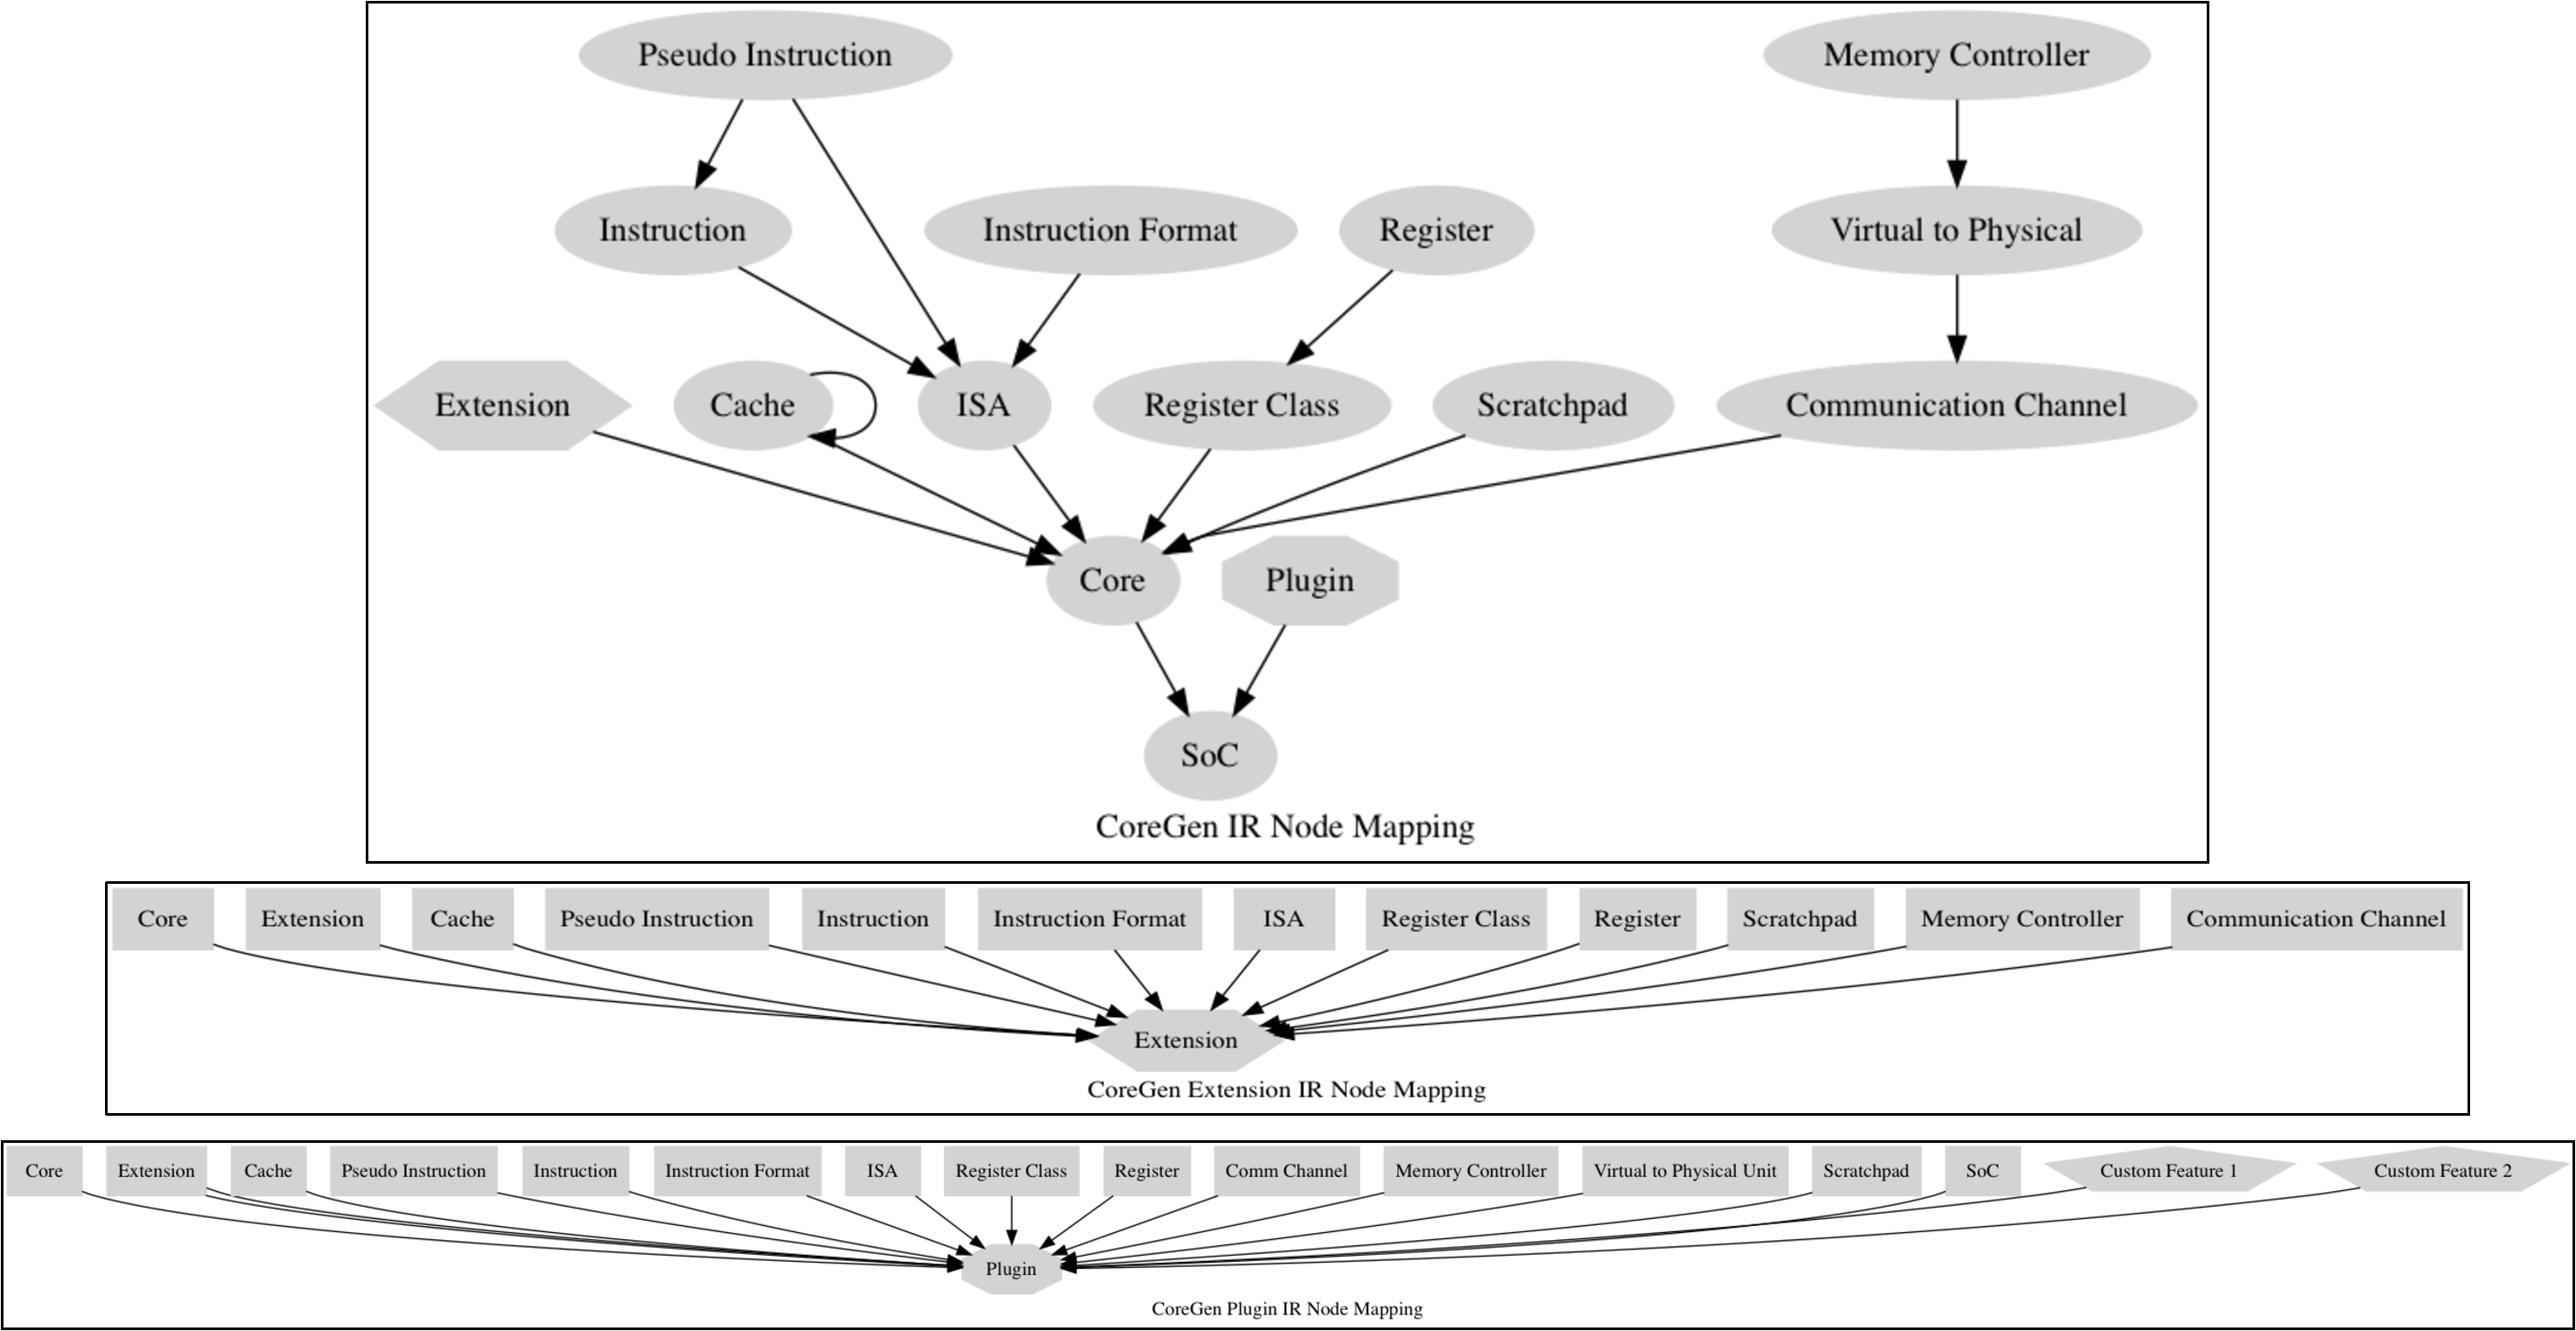
\includegraphics[width=\textwidth]{figures/NodeMapping.pdf}
\vspace*{8pt}
\caption{CoreGen IR Node Hierarchy}
\label{fig:IRNodes}
\end{center}
\end{figure}

Each of the aforementioned node types follows are predefined hierarchy and dependence profile.  We represent 
these dependencies in Figure~\ref{fig:IRNodes}.  The dependencies are maintained via the standard CoreGen IR 
formatting.  As a result, dependencies are naturally expressed in the IR.

The two exceptions to this rule are \textit{Extensions} and \textit{Plugins}.  These can effectively fall anywhere within the 
IR hierarchy.  Further, both extensions and plugins can contain dependent nodes within themselves in order to express 
additional information.  We will further see how these function in Sections~\ref{sec:ExtensionNodes} and~\ref{sec:PluginNodes}.  

\clearpage
%\subsection{Definitions}

%\label{definitions}
%\begin{description}
%\item[Stoichiometry]
%The relationship between the relative quantities of substances taking part in a reaction or forming a compound, typically a ratio of whole integers.
%\item[Atomic mass]
%The mass of an atom of a chemical element expressed in atomic mass units. It is approximately equivalent to the number of protons and neutrons in %the atom (the mass number) or to the average number allowing for the relative abundances of different isotopes. 
%\end{description} 

\subsection{Required Packages and Manipulating IR}

Given the textual nature of the CoreGen intermediate representation, there are no external 
packages required to read and/or write the IR.  However, we \textit{highly} recommend that 
you utilize the integrated CoreGen tooling in order to maintain the internal dependencies and 
verify the syntactical correctness of the IR.  Further, parsing the YAML using non-CoreGen 
tools may result in unresolved internal dependency links due to incorrect parsing order.  
Regardless of the format of the IR text, the CoreGen tools will parse the file in the correct nodal 
order.  

 
%----------------------------------------------------------------------------------------
%	SECTION 2
%----------------------------------------------------------------------------------------
\clearpage
\section{CoreGen IR Nodes}
\label{sec:CoreGenIRNodes}

In this section, we outline how each individual node type is constructed, how they link 
to other nodes and the syntactical definitions utilized therein.  Each section describes 
the generic format of the node.  The sequences and sequence elements will include 
scalar values in one of the following types (Table~\ref{tab:scalartypes}):

\begin{table}[h]
\begin{center}
\caption{CoreGen IR Scalar Types}
\vspace{0.125in}
\label{tab:scalartypes}
\begin{tabular}{|c|l|}
\hline
\textbf{Type} & \textbf{Description}\\
\hline
\multirow{2}{*}{\textbf{\texttt{String}}} & Strings are utilized to represent names and references to names.\\
					                   & In some instances, Strings are used to represent special object types.\\
\hline
\multirow{2}{*}{\textbf{\texttt{Bool}}} & Bool values are utilized to represent pure booleans.\\
                                                               & They can be either \texttt{true} or \texttt{false}.\\
\hline
\multirow{2}{*}{\textbf{\texttt{Integer}}} & Integer values are utilized to represent indices and basic parameter values.\\
                                                                   & Where appropriate, we indicate the perceived types.\\
\hline
\multirow{2}{*}{\textbf{\texttt{Special}}} & Special objects a textual keywords used to trigger specific architectural features.\\
                                                                     & These are represented as: \texttt{\{Value1,Value2,...\}}.\\
\hline
\end{tabular}
\end{center}
\end{table}  

\subsection{Node Names and Linkage}
\label{sec:NameNamesAndLinkage}

Each IR node in the CoreGen IR format has a unique name that represents a unique hardware object.  Names must be 
unique across all IR nodes.  We require unique names as the respective node names are utilized to link nodes in a 
dependent manner across the design.  For example, a \texttt{core} node may have a dependent \texttt{cache} node.  We provide 
an example node dependency using these names in Listing~\ref{lis:nodenames}.  Notice how we define an instruction node (\texttt{TEST54.inst0}) 
and a pseudo instruction node (\texttt{TEST54.pinst0}) that depends upon the core instruction by name.

Given this use of textual names in the IR, we must define a valid naming convention that is preserved in the IR.  The valid node 
name rules are listed as follows: 

\begin{itemize}
\item Names must be non null (\textit{length greater than 0})
\item Names must begin with an alpha character (\textit{[a-z,A-Z]})
\item Names must contain only alphanumeric characters and periods (\textit{[a-z,A-Z,0-9,.]})
\item Names are case sensitive, but can include any combination of upper and lower case characters
\end{itemize}

Example valid and invalid node names are listed in Table~\ref{tab:validinvalidnames}.  

\begin{table}[h]
\begin{center}
\caption{CoreGen IR Valid and Invalid Node Names}
\vspace{0.125in}
\label{tab:validinvalidnames}
\begin{tabular}{|c|c|l}
\hline
\textbf{Valid} & \textbf{Invalid}\\
\hline
nodename, NodeName, nodeName0, Node.Name.9 & 9Name, Node\&Name, \%NodeName\\
\hline
\end{tabular}
\end{center}
\end{table} 

\clearpage
\vspace{0.125in}
\begin{lstlisting}[frame=single,style=base,showstringspaces=false,caption={Node Naming and Linkage},captionpos=b,label={lis:nodenames}]
Insts:
  - Inst: @TEST54.inst0@
    ISA: TEST54.isa
    InstFormat: TEST54.if
    Encodings:
      - EncodingField: opcode
        EncodingWidth: 8
        EncodingValue: 1
PseudoInsts:
  - PseudoInst: TEST54.pinst0
    ISA: TEST54.isa
    Inst: @TEST54.inst0@
    Encodings:
      - EncodingField: RA
        EncodingWidth: 8
        EncodingValue: 0
\end{lstlisting}  

\subsection{User Defined RTL}
\label{sec:UserDefinedRTL}

For each of the forthcoming node types, users have the ability to override the 
default CoreGen code generation facilities in order to include custom RTL.  Currently, 
The CoreGen IR specification permits users to utilize this feature in two ways.  First, 
users have the ability to define inline RTL.  This RTL can currently be written in either 
Chisel (Chisel 3) or Verilog.  Inline RTL must follow the naming conventions and port 
definitions supported by the CoreGen code generation facilities (NEED REFERENCE).  
An example of defining inline RTL for a single instruction in Chisel3 is shown in Listing~\ref{lis:inlinertl}.  
Notice how the inline RTL source code is quoted.  For each inline RTL sample provided with the 
CoreGen node, you must also specify the \texttt{RTLType}.  Types can be one of \texttt{Chisel}, 
\texttt{Verilog} and \texttt{Unknown}.    

\vspace{0.125in}
\begin{lstlisting}[frame=single,style=base,showstringspaces=false,caption={Sample Inline RTL},captionpos=b,label={lis:inlinertl}]
Insts:
  - Inst: TEST69.inst0
    ISA: TEST69.isa
    InstFormat: TEST69.if
    Encodings:
      - EncodingField: opcode
        EncodingWidth: 8
        EncodingValue: 1
    @RTL: "when( RA === 0x05){
            RT = RA << RB
          } .otherwise {
            RT = RA >> RB
          }"@
     @RTLType: Chisel@
\end{lstlisting}  

The second path by which users may override a default node using RTL is by utilizing an external 
RTL file.  By utilizing the \texttt{RTLFile} parameter with any node, the user may specify an external 
RTL file that is managed outside of CoreGen and its constituent tools.  Take note that the external RTL 
file is relative to the project path utilized by the CoreGen tools.  An example of doing so is shown in 
Listing~\ref{lis:externalrtl}.  

\clearpage
\vspace{0.125in}
\begin{lstlisting}[frame=single,style=base,caption={Sample External RTL File},captionpos=b,label={lis:externalrtl}]
Insts:
  - Inst: TEST69.inst0
    ISA: TEST69.isa
    InstFormat: TEST69.if
    Encodings:
      - EncodingField: opcode
        EncodingWidth: 8
        EncodingValue: 1
    @RTLFile: Sample.v@
    @RTLType: Verilog@
\end{lstlisting}


\clearpage
\subsection{Node Override}
\label{sec:NodeOverride}

In addition to providing the ability to override each node with user-defined RTL, the CoreGen IR infrastructure 
also provides the ability to override an entire node's construction with user-defined logic.  This mechanism is analogous 
to utilizing templates in modern object-oriented programming models.  Users have the ability to utilize \textit{plugins} to override 
the default behavior and/or define non-standard features for a target IR node.  This feature can also be utilized to integrate pre-existing 
hardware IP into new designs.  This functionality 
can be performed on all nodes except plugins, extensions, encoding and pseudo instructions.  

An example of utilizing this feature is provided in Listing~\ref{lis:nodeoverride}.  The first step in this process is to define a plugin node 
that will be utilized to override the default functionality of a standard node.  In this case, we utilize a pre-existing \texttt{CacheLayerPlugin} 
and define a \texttt{CachePlugin} node.  This theoretical plugin node instantiates an \textit{N}-level cache with pre-existing IP where the number 
of cache levels is defined by a custom feature (\texttt{Levels}).  With this plugin node defined, we can now define a base cache node defined 
as the \texttt{L0.Cache}.  Within this cache node, we use the \texttt{Override} keyword and attach the plugin node definition that we previously 
defined (\texttt{CachePlugin}).  Note that you \textbf{must} utilize the plugin node name (\texttt{Plugin}), not the actual name of the plugin 
implementation (\texttt{PluginName}).  The CoreGen IR supports multiple instantiations of the same plugin implementation under different names.  
This permits users to re-use existing IP and define unique features for each instance of the plugin.  
For more information regarding the definition and construction of the actual \texttt{Plugin} nodes, see Section~\ref{sec:PluginNodes}.  

\vspace{0.125in}
\begin{lstlisting}[frame=single,style=base,showstringspaces=false,caption={Sample Node Override},captionpos=b,label={lis:nodeoverride}]
Plugins:
  - Plugin: @CachePlugin@
    PluginName: CacheLayerPlugin
    MajorVersion: 1
    MinorVersion: 0
    PatchVersion: 0
    Features:
    - FeatureName: Levels
      FeatureType: unsigned
      FeatureValue: 3
Caches:
  - Cache: L0.Cache
    Sets: 1024
    Ways: 8
    Override: @CachePlugin@
\end{lstlisting}  

\clearpage
\subsection{Node Notes}
\label{sec:NodeNotes}

Each node has an additional attribute that permits users to add specific \textit{notes} or comments 
for future reference.  These \texttt{Notes} fields do not affect the overall functionality, stability 
or connectivity of the constituent design.  Rather, these attributes may be utilized, queried or 
processed by downstream tools.  For example, the CoreGen \textit{SpecDoc} pass utilizes these notes
to output specific information for constituent design elements.  An example of doing so is shown 
in Listing~\ref{lis:notes}.

\vspace{0.125in}
\begin{lstlisting}[frame=single,style=base,caption={Sample Node Notes},captionpos=b,label={lis:notes}]
Insts:
  - Inst: TEST69.inst0
    ISA: TEST69.isa
    InstFormat: TEST69.if
    Encodings:
      - EncodingField: opcode
        EncodingWidth: 8
        EncodingValue: 1
    @Notes: This instruction performs carry-less addition.@
\end{lstlisting}


\clearpage
\subsection{Projects}
\label{sec:ProjectNodes}

CoreGen IR files may provide an optional project definition block.  This block of IR does not contain any 
dependencies with other IR nodes.  Rather,  it is designed to provide tools with additional information regarding 
the location and target function of the IR contained therein.  Project nodes are utilized to define project names, 
paths, project types and Chisel output versions.  Currently, we support four disparate project types as show in 
Table~\ref{tab:ProjTypes}.   

\begin{table}[h]
\begin{center}
\caption{CoreGen Project Types}
\vspace{0.125in}
\label{tab:ProjTypes}
\begin{tabular}{|c|l|}
\hline
\textbf{Parameter} & \textbf{Description}\\
\hline
\texttt{soc} & System on chip projects are full designs with deep hierarchies of nodes\\
\hline
\multirow{2}{*}{\texttt{module}} & Module projects are designed to be very compact hierarchies of nodes\\
                                                       & potentially with custom RTL\\
\hline
\multirow{2}{*}{\texttt{extension}} & Extension projects encapsulate a single block of extension IR nodes\\
                                                           & to be utilized in other projects\\
\hline
\texttt{unknown} & All other projects fall into the \textit{unknown} category\\
\hline
\end{tabular}
\end{center}
\end{table} 

We see an example block of project node IR in Listing~\ref{lis:projectnode}.  

\vspace{0.125in}
\begin{lstlisting}[frame=single,style=base,caption={Project Node Definition},captionpos=b,label={lis:projectnode}]
ProjectInfo:
  - ProjectName: @String@
    ProjectRoot: @String@
    ProjectType: @Special@
    ChiselMajorVersion: @Integer@
    ChiselMinorVersion: @Integer@
\end{lstlisting} 

\clearpage
\subsection{Registers}
\label{sec:RegisterNodes}

Register nodes define a single instance of a register in hardware.  Registers may also have named aliases, referred 
to as a \texttt{PseudoName}.  Further, subregisters (\texttt{SubRegs}) can be defined whereby a unique pseudoname 
is utilized to access a specific portion of the parent register.  For example, if we define a parent register \textit{FOO} 
with a width of 64 bits, we may also define a \texttt{SubReg} \textit{FOO.BAR} to alias bits \texttt{[31-0]} (the lower 
half of the register).  

Additional parameters are described in Table~\ref{tab:RegNodeParams}.  We provide a sample register IR block in Listing~\ref{lis:registernode}.  

\begin{table}[h]
\begin{center}
\caption{CoreGen Register Node Parameters}
\vspace{0.125in}
\label{tab:RegNodeParams}
\begin{tabular}{|c|l|}
\hline
\textbf{Parameter} & \textbf{Description}\\
\hline
\texttt{Width} & Defines the width (in bits) of the register. (Int)\\
\hline
\texttt{Index} & Defines the index value of the register. (Int)\\
\hline
\texttt{PseudoName} & [Optional] Defines a register pseudo name (String)\\
\hline
\multirow{2}{*}{\texttt{IsFixedValue}} & Sets a parameter indicating that the register has\\
                                                                 & a read-only, fixed value. (Bool).\\
\hline
\multirow{2}{*}{\texttt{IsSIMD}} & Sets a parameter indicating that the register is a SIMD register.\\
                                                       & The register width must encapsulate the entire SIMD block. (Bool)\\
\hline
\multirow{2}{*}{\texttt{RWReg}} & Sets a parameter indicating that the register is a read-write register\\&(Bool)\\
\hline
\multirow{2}{*}{\texttt{ROReg}} & Sets a parameter indicating that the register is a read-write register\\
                                                       & Cannot be \texttt{true} if RWReg is \texttt{true}. (Bool)\\
\hline
\multirow{2}{*}{\texttt{CSRReg}} & Sets a parameter indicating that the register is a control status register.\\
                                                          & This can be read-only or read-write. (Bool)\\
\hline
\multirow{2}{*}{\texttt{AMSReg}} & Sets a parameter indicating that the register is an arithmetic machine state register.\\
                                                          & The hardware code generator will integrate these into the pipeline. (Bool)\\
\hline
\multirow{2}{*}{\texttt{TUSReg}} & Sets a parameter indicating that the register is shared across all thread units within the core.\\
                                                          & Either \texttt{Shared} or \texttt{TUSReg} can be set, but not both. (Bool)\\
\hline
\multirow{2}{*}{\texttt{PCReg}} & Sets a parameter indicating that the register is designated as a program counter.\\
                                                          & This attribute may only exist in a single register per instruction set.  (Bool)\\
\hline
\multirow{2}{*}{\texttt{Shared}} & Sets a parameter indicating that the register is a shared register.\\
                                                          & The hardware generator will create \textbf{ONE} instance of the register for all cores. (Bool)\\
\hline
\multirow{2}{*}{\textbf{SubRegs}} & \\ & \\
\hline
\multirow{2}{*}{\texttt{SubReg}} & Sets the unique subregister name.\\
                                                          & The name must be unique across all registers within the register class (String)\\
\hline
\multirow{2}{*}{\texttt{StartBit}} & Sets the starting bit position of the subregister in the parent register.\\
                                                          & The start bit must be less than the end bit and a minimum of one bit. (Int)\\
\hline
\multirow{2}{*}{\texttt{EndBit}} & Sets the ending bit position of the subregister in the parent register.\\
                                                          & The end bit must be greater than the start bit and a minimum of one bit (Int)\\
\hline
\end{tabular}
\end{center}
\end{table}  

\clearpage
\vspace{0.125in}
\begin{lstlisting}[frame=single,style=base,caption={Register Node Definition},captionpos=b,label={lis:registernode}]
Registers:
  - RegName: @String@
    Width: @Integer@
    Index: @Integer@
    PseudoName: @String@
    IsFixedValue: @Bool@
    IsSIMD: @Bool@
    RWReg: @Bool@
    ROReg: @Bool@
    CSRReg: @Bool@
    AMSReg: @Bool@
    TUSReg: @Bool@
    PCReg: @Bool@
    Shared: @Bool@
    SubRegs:
      - SubReg: @String@
        StartBit: @Integer@
        EndBit: @Integer@
      - SubReg: @String@
        StartBit: @Integer@
        EndBit: @Integer@
  - RegName: @String@
    Width: @Integer@
    Index: @Integer@
    PseudoName: @String@
    IsFixedValue: @Bool@
    IsSIMD: @Bool@
    RWReg: @Bool@
    ROReg: @Bool@
    CSRReg: @Bool@
    AMSReg: @Bool@
    TUSReg: @Bool@
    Shared: @Bool@
   ...more registers
\end{lstlisting}  

\clearpage
\subsection{Register Classes}
\label{sec:RegisterClassNodes}

Register class nodes define an instance of a register file.  The register file will contain some number of registers, each of 
which may have specific attributes.  Indexing into the register file is defined by the registers contained therein and \textit{does not} 
need to be monotonically increasing.  Despite the ability to registers within the same register file that have disparate attributes, 
the HDL code generation mechanisms in CoreGen will select the largest bit width register in order to determine the space requirements 
of the register file.  As a result, if the design requires several different sizes of registers, it is advantageous to separate them into distinct 
register files for the purpose of optimizing the eventual RTL.  

Register classes are defined by two parameters: the register class name and the registers that exist within the register class.  The registers 
defined in the register class are references to register defined in the register node section (See Section~\ref{sec:RegisterNodes}).   The 
register naming convention must match that of the defined registers.  We provide a sample register class 
IR block in Listing~\ref{lis:regclassnode}. 

\vspace{0.125in}
\begin{lstlisting}[frame=single,style=base,caption={Register Class Node Definition},captionpos=b,label={lis:regclassnode}]
RegClasses:
  - RegisterClassName: @String@
    Registers:
      - @String@
      - @String@
      - @String@
  - RegisterClassName: @String@
    Registers:
      - @String@
      - @String@
      - @String@
  ...more reg classes
\end{lstlisting} 

\clearpage
\subsection{Instruction Sets}
\label{sec:InstructionSetNodes}

Instruction set nodes are effectively container nodes.  They are designated as a container for multiple 
instructions and instruction formats.  As a result, the only parameter utilized to identify an individual 
instruction set is its respective name.  Designs may have any number of instruction sets.  We provide an 
example instruction set IR block in Listing~\ref{lis:isa}.  

\vspace{0.125in}
\begin{lstlisting}[frame=single,style=base,caption={Instruction Set Node Definition},captionpos=b,label={lis:isa}]
ISAs:
  - ISAName: @String@
  - ISAName: @String@
\end{lstlisting}

\clearpage
\subsection{Instruction Formats}
\label{sec:InstructionFormatNodes}

The instruction format nodes define the formatting information, including field types, field widths and required 
information for each instruction format in \textbf{little endian}.  The instruction format nodes do not define the actual instructions, only 
the encoding formats.  Instruction formats can contain any number of instruction fields.  The minimum field 
width is a single bit.  The maximum field width is equivalent to the entire width of the instruction format (\texttt{FormatWidth}).  

Each width must be designated as one of three potential field types.  For register fields, you \textbf{must} also 
specify the target register class that is associated with the field (\texttt{RegClass}).  Note that the width of the 
field should encapsulate the maximum potential index for the target register class.  For instruction code fields, 
the width of the field will define the number of encodings.

Finally, instruction encodings are not required to contain contiguous fields.  You may opt to leave undefined 
space between fields.  The width of the encoding must match the largest ending bit field.  For example, if 
your instruction format has the last field defined to end on bit 31 (\texttt{EndBit}), then your entire encoding must be at least 
32 bits.   

\begin{table}[h]
\begin{center}
\caption{CoreGen Instruction Format Node Parameters}
\vspace{0.125in}
\label{tab:InstFormatParams}
\begin{tabular}{|c|l|}
\hline
\textbf{Parameter} & \textbf{Description}\\
\hline
\texttt{ISA} & Defines the instruction set architecture container. (String)\\
\hline
\texttt{FormatWidth} & Defines the width (in bits) of the register. (Int)\\
\hline
\hline
\textbf{Fields} & \\
\hline
\texttt{FieldName} & Defines the name of the respective field. (String)\\
\hline
\multirow{4}{*}{\texttt{FieldType}} & Defines the field type.  This must be one of the following. (Special)\\
                                                            & \texttt{CGInstReg} : Defines a register field.  Requires \texttt{RegClass} be defined.\\
                                                            & \texttt{CGInstCode} : Defines an instruction code (opcode, function code, etc).\\
                                                            & \texttt{CGInstImm} : Defines a field for an immediate value.\\
\hline
\texttt{FieldWidth} & Defines the width of the instruction field. (Integer)\\
\hline
\texttt{StartBit} & Defines the starting bit position of the field. (Integer)\\
\hline
\texttt{EndBit} & Defines the end bit position of the field. (Integer)\\
\hline
\texttt{MandatoryField} & Determines whether the field \textbf{must} be defined by the implementing instruction. (Bool)\\
\hline
\multirow{2}{*}{\texttt{RegClass}} & Sets the target register class parameter for \texttt{CGInstReg} fields.  (String)\\ & \\
\hline
\end{tabular}
\end{center}
\end{table} 

We provide an example Instruction Format IR block in Listing~\ref{lis:instformat}.  

\vspace{0.125in}
\begin{lstlisting}[frame=single,style=base,caption={Instruction Format Node Definition},captionpos=b,label={lis:instformat}]
InstFormats:
  - InstFormatName: @String@
    ISA: @String@
    FormatWidth: @Integer@
    Fields:
      - FieldName: @String@
        FieldType: @{CGInstReg, CGInstCode, CGInstImm}@
        FieldWidth: @Integer@
        StartBit: @Integer@
        EndBit: @Integer@
        MandatoryField: @Bool@
      - FieldName: @String@
        FieldType: @{CGInstReg, CGInstCode, CGInstImm}@
        FieldWidth: @Integer@
        StartBit: @Integer@
        EndBit: @Integer@
        MandatoryField: @Bool@
        RegClass: @String@
      - FieldName: @String@
        FieldType: @{CGInstReg, CGInstCode, CGInstImm}@
        FieldWidth: @Integer@
        StartBit: @Integer@
        EndBit: @Integer@
        MandatoryField: @Bool@
        RegClass: @String@
      - FieldName: @String@
        FieldType: @{CGInstReg, CGInstCode, CGInstImm}@
        FieldWidth: @Integer@
        StartBit: @Integer@
        EndBit: @Integer@
        MandatoryField: @Bool@
        RegClass: @String@
\end{lstlisting}

\clearpage
\subsection{Instructions}
\label{sec:InstructionNodes}

Instruction nodes represent individual instances of single instructions.  Each instruction 
node is attached to an instruction set reference as well as a specific instruction format.  In addition 
to the aforementioned references, each instruction has the ability to include any necessary encoding 
information as well.  A single instruction can define multiple encoding blocks, each with specific 
encoding information that is mapped back to an individual named field in the instruction format.  For example, 
if the instruction format has a field called \textit{opcode} that has the \texttt{MandatoryField} flag set to \texttt{true}, 
the instruction node may have an \texttt{Encoding} definition with the respective value for that instruction.  

Note that it is up to the user to avoid collisions in the encodings across multiple instructions.  The CoreGen tools 
may provide IR passes that check for these idiosyncracies, but the IR does not inherently prohibit collisions.  Further, 
encoding definitions require that the user specify the encoding width (\texttt{EncodingWidth}).  For opcode fields, this 
should be set to the same width as defined in the instruction encoding (\texttt{FieldWidth}).  However, for fields such 
as immediate values, setting this width to something less than the full field width with automatically truncate the value 
to what is specified.  For example, if the instruction encoding field for the immediate is 16 bits, but you define an instruction 
with a 12 bit immediate, the value in the immediate field of that instruction will be truncated to 12 bits.

Each instruction nodes can also drive the syntax by which the compiler's assembly code is generated and parsed.  The 
\texttt{Syntax} field contains a string value in a specific format that defines the instruction mnemonics and associated 
syntax that is utilized to construct the associated assembler and disassembler.  This syntax is constructed in a specific 
manner such that the CoreGen infrastructure has the ability to match the respective mnemonic to the correct instruction 
format field.  The syntax must include the instruction name (which may differ from the instruction node name) and some 
number arguments.  The argument names must match the respective register class or immediate field names 
of the respective instruction format.  Register class arguments are delineated with \textit{\%} characters and immediate 
arguments are delineated with \textit{\$} characters.  User may also intersperse commas and parenthesis throughout the syntax at will.

For example, consider an instruction \texttt{ADD} whose instruction format has three register class fields: \texttt{RT}, \texttt{RA} and 
\texttt{RB}.  We may specify the instruction syntax as follows: \texttt{ADD \%RT, \%RA, \%RB}.  We may also have an additional 
instruction, \texttt{LOAD}, whose instruction format contains two register class fields (\texttt{RT}, \texttt{RA}) and a single immediate 
field (\texttt{IMM}).  Our instruction syntax may then be formatted as: \texttt{LOAD \%RT, \$IMM(\%RA)}.  Note the use of the preceding 
characters for the register class and immediate field designators.    

Finally, instructions have the ability to include inline StoneCutter definitions for each instruction (NEED REFERENCE).  These 
inline StoneCutter instruction definitions are compiled consolidated into larger StoneCutter source files using the CoreGen 
infrastructure and subsequently compiled into Chisel HDL.  Inline StoneCutter language is designated using \texttt{Impl} 
attributes within an individual instruction definition.   

We provide an example instruction node in Listing~\ref{lis:inst}.     
\clearpage
\vspace{0.125in}
\begin{lstlisting}[frame=single,style=base,caption={Instruction Node Definition},captionpos=b,label={lis:inst}]
Insts:
  - Inst: @String@
    ISA: @String@
    InstFormat: @String@
    Syntax: @String@
    Encodings:
      - EncodingField: @String@
        EncodingWidth: @Integer@
        EncodingValue: @Integer@
  - Inst: @String@
    ISA: @String@
    InstFormat: @String@
    Syntax: @String@
    Encodings:
      - EncodingField: @String@
        EncodingWidth: @Integer@
        EncodingValue: @Integer@
    Impl: @String@
\end{lstlisting}

\clearpage
\subsection{Pseudo Instructions}
\label{sec:PseudoInstructionNodes}

Pseudo instruction nodes are special types of instruction nodes.  They do not represent actual instructions.  Rather, 
pseudo instructions contain special encoding directions for previously defined instructions and/or new instruction names.  
For example, in traditional RISC architectures register moves are implemented as unsigned addition instructions whereby 
the immediate values are set to zero.  An example of this is noted as follows: 

\vspace{0.125in}
\begin{verbatim}
#  register R0 = zero
add r10, r11, r0  # R10 = R11+R0
mov r10, r11      # Pseudo instruction for 'add r10, r11, r0'
\end{verbatim}

Pseudo instructions require a unique name, the associated ISA and the target instruction that you seek to alias.  
You must also define a set of encoding parameters that are utilized to incorporate specific encodings for specific fields.  
For example, if you seek to define a pseudo instruction whereby an individual register file is always set to the same 
register index, utilize a pseudo instruction with an encoding field.  Further, much like the original instruction definition, pseudo 
instructions permit the user to define assembly mnemonics that are echoed in the compiler implementation.  The assembly 
mnemonics follow the syntax rules defined in Section~\ref{sec:InstructionNodes}.  An example set of pseudo instructions is provided 
in Listing~\ref{lis:pseudoinst}.  

\vspace{0.125in}
\begin{lstlisting}[frame=single,style=base,caption={Pseudo Instruction Node Definition},captionpos=b,label={lis:pseudoinst}]
PseudoInsts:
  - PseudoInst: @String@
    ISA: @String@
    Inst: @String@
    Encodings:
      - EncodingField: @String@
        EncodingWidth: @Integer@
        EncodingValue: @Integer@
    Syntax: @String@
  - PseudoInst: @String@
    ISA: @String@
    Inst: @String@
    Encodings:
      - EncodingField: @String@
        EncodingWidth: @Integer@
        EncodingValue: @Integer@
    Syntax: @String@
\end{lstlisting}

\clearpage
\subsection{Caches}
\label{sec:CacheNodes}

Cache nodes represent a single level of a traditional cache hierarchy.  Regardless of whether the target use is 
designated as an instruction cache, data cache or otherwise, the cache node is defined in the same manner.  
The target use is determined by how the cache is connected to the core (or cores).  Cache nodes are required 
to have at least two parameters: \texttt{Sets} and \texttt{Ways}.  These represent the number of cache sets 
and the number of \textit{ways} are represented in the cache.

Caches can also be configured in hierarchies.  Each level in the cache must be defined as a cache node.  To define 
a cache hierarchy, start with the cache layer closest to the core (usually defined as the \textit{L1} layer) and add a 
\texttt{SubLevel} to the cache.  The sublevel defines a connection to the next layer in the cache hierarchy.  Nodes 
may exist as parents (sublevel to a lower level cache) and as a parent (contain a sublevel).  You may define any 
number of caching layers providing that the connectivity is present between layers.  An example caching hierarchy 
is providing in Listing~\ref{lis:cache}.  

\vspace{0.125in}
\begin{lstlisting}[frame=single,style=base,caption={Cache Node Definition},captionpos=b,label={lis:cache}]
Caches:
  - Cache: @String@
    Sets: @Integer@
    Ways: @Integer@
  - Cache: @String@
    Sets: @Integer@
    Ways: @Integer@
    SubLevel: @String@
  - Cache: @String@
    Sets: @Integer@
    Ways: @Integer@
\end{lstlisting}

\clearpage
\subsection{Scratchpad Memories}
\label{sec:Spads}

Scratchpad nodes are utilized to represent special case memory nodes that reside 
on die (as opposed to external memories such as DRAM).  Further, these memory 
nodes participate in the normal addressing mechanisms, unlike cache hierarchies 
which are implied as a part of the memory pipeline.  

Scratchpad nodes can be unique for individual cores or attached to multiple cores or other 
nodes.  Each scratchpad memory node must include the size of the scratchpad (\texttt{MemSize}), 
the number of request ports (\texttt{RqstPorts}), the number of response ports (\texttt{RspPorts}) 
and the starting address (\texttt{StartAddr}).  The total address space provided by the individual scratchpad 
is \textit{StartAddr + MemSize}.  Note that individual scratchpads may have the same address space providing that 
they are not connected to the same core.  Further, multiple scratchpads can be connected to individual cores 
providing that the address spaces do not collide.  An example scratchpad node definition is provided in Listing~\ref{lis:spad}.    

\vspace{0.125in}
\begin{lstlisting}[frame=single,style=base,caption={Scratchpad Node Definition},captionpos=b,label={lis:spad}]
Scratchpads:
  - Scratchpad: @String@
    MemSize: @Integer@
    RqstPorts: @Integer@
    RspPorts: @Integer@
    StartAddr: @Integer@
  - Scratchpad: @String@
    MemSize: @Integer@
    RqstPorts: @Integer@
    RspPorts: @Integer@
    StartAddr: @Integer@
\end{lstlisting}

\clearpage
\subsection{Virtual to Physical Translation Units}
\label{sec:VTOPNodes}

The virtual to physical (\textit{VTP}) nodes include the ability to perform virtual to physical memory address 
translation in conjunction with the backend memory controller and scratchpad memory nodes.  Currently, 
the VTP nodes require a single parameter, the name of the VTP node.  Note that it may be inherently dangerous 
to have multiple VTP nodes in a single design without sufficient separation.  For example, a heterogeneous design 
that contains multiple, tightly integrated cores may still have a single VTP node.  However, a design that includes 
a loosely connected accelerator (with its own constituent memory controller) may perform its own virtual to physical 
translation.  An example of the VTP node syntax is shown in Listing~\ref{lis:vtp}.  

\vspace{0.125in}
\begin{lstlisting}[frame=single,style=base,caption={VTP Node Definition},captionpos=b,label={lis:vtp}]
VTPControllers:
  - VTP: @String@
\end{lstlisting}

\clearpage
\subsection{Memory Controllers}
\label{sec:MemCtrlNodes}

Memory controller nodes are designed to receive physical addresses from upstream devices.  The memory controller 
subsequently transfer the requests to the external memory devices.  Many designs may warrant overriding these nodes 
with external RTL IP given design-specific external memory requirements.  Otherwise, memory controller nodes require 
a unique node name as well as the number of upstream memory ports.  Currently, the number of ports (\texttt{Ports}) should be an even 
number as these are divided evenly between request ports and response ports.  An example memory controller IR block is 
shown in Listing~\ref{lis:mctrl}.  

\vspace{0.125in}
\begin{lstlisting}[frame=single,style=base,caption={Memory Controller Node Definition},captionpos=b,label={lis:mctrl}]
MemoryControllers:
  - MemoryController: @String@
    Ports: @Integer@
  - MemoryController: @String@
    Ports: @Integer@
\end{lstlisting}

\clearpage
\subsection{Communication Channels}
\label{sec:CommNodes}

Communication nodes provide connectivity between disparate nodes that would otherwise have no implied 
connectivity.  For example, if you connect a cache node to a core, there is an implied link via the memory pipeline.  However, 
if you connect a set of cores together (via a bus or other topology), there is no implication of how they may communicate.  
Communication nodes are utilized to connect various nodes or groups of nodes together into a singular topology.  Nodes may 
include connectivity between multiple communication nodes in different networks.  For example, a core may include connectivity 
to four adjacent cores in order to form a on-chip mesh interconnect.  

Communication nodes require four main parameters as noted in Table~\ref{tab:CommParams}.  We show an example Communication 
node in Listing~\ref{lis:comm}.    

\begin{table}[h]
\begin{center}
\caption{CoreGen Instruction Format Node Parameters}
\vspace{0.125in}
\label{tab:CommParams}
\begin{tabular}{|c|l|}
\hline
\textbf{Parameter} & \textbf{Description}\\
\hline
\texttt{Comm} & Defines the unique name of the communication node. (String)\\
\hline
\multirow{6}{*}{\texttt{Type}} & Defines the communication node type.  This must be one of the following. (Special)\\
                                                   & \texttt{P2P} : Defines a peer-to-peer communication channel for two node endpoints.\\
					    & \texttt{Bus} : Defines a bus communication channel with min 2 endpoints and no maximum.\\
					    & \texttt{NOC} : Defines a network on chip communication channel with\\
					    & min 2 endpoints and no maximum.\\
					    & \texttt{Unknown} : User-defined communication channel that requires user-provided RTL.\\
\hline
\multirow{2}{*}{\texttt{Endpoints}} & This contains a sequenced list of endpoint nodes that\\
                                                            & are connected to the communication channel.\\
\hline
\end{tabular}
\end{center}
\end{table}

\vspace{0.125in}
\begin{lstlisting}[frame=single,style=base,caption={Communication Node Definition},captionpos=b,label={lis:comm}]
Comms:
  - Comm: @String@
    Type: @{P2P,Bus,NOC,Unknown}@
    Width: @Integer@
    Endpoints:
      - @String@
      - @String@
      - @String@
\end{lstlisting}

\clearpage
\subsection{Cores}
\label{sec:CoreNodes}

Core nodes define a single instance of a traditional "core".  This includes arithmetic facilities, register files 
and any required encoding data (instruction formats, register indices, etc).  Each core node must include 
an associated instruction set definition (\texttt{ISA}), any required register classes for the target ISA (\texttt{RegisterClasses}) 
and optionally, one or more cache units.  While caching units are optional dependent nodes for a core, we 
highly recommend that cores have at least an instruction cache facility.  Otherwise, the instruction fetch 
performance of the core will be very poor.  

In addition to the aforementioned base nodes, cores can be augmented with one or more extensions.  These extensions 
may include additional, registers, register classes or other non-standard nodes beyond what is defined in the base 
core infrastructure.

Core nodes may also define the degree of symmetric multithreading (SMT) by specifying the number of \texttt{ThreadUnits}.  
This optional keyword permits users to specify the number of unique thread units for the respective core.  The hardware 
code generator will output unique register files for each thread unit unless a register has been designated as 
\textit{thread unit shared} (\texttt{TUSReg}) or \texttt{Shared}.  See Section~\ref{sec:RegisterNodes} for descriptions 
of these register attributes.    
The code generator will not, however, output unique \texttt{Extensions} for each thread unit.  
A single instance of a shared register will be generated and shared across the cores.  If not specified, the number of 
\texttt{ThreadUnits} is assumed to be \textit{1}.  

We see an example of a basic and extended core node in Listing~\ref{lis:core}.   

\vspace{0.125in}
\begin{lstlisting}[frame=single,style=base,caption={Core Node Definition},captionpos=b,label={lis:core}]
- Core: @String@
    Cache: @String@
    ISA: @String@
    ThreadUnits: @2@
    RegisterClasses:
      - RegClass: @String@
      - RegClass: @String@
  - Core: @String@
    Cache: @String@
    ISA: @String@
    RegisterClasses:
      - RegClass: @String@
      - RegClass: @String@
    Extensions:
      - Extension: @String@
\end{lstlisting}

\clearpage
\subsection{SoCs}
\label{sec:SoCNodes}

SoC (or \textit{System on Chip}) nodes are top-level, container nodes that are utilized to tie multiple cores and their dependent 
nodes together into a single package.  Generally speaking, there should be only a single SoC node in a design.  It is possible to 
have multiple SoC nodes in a given IR file, but the CoreGen pass infrastructure will likely flag this as being potentially erroneous.  
For each SoC node, you must define some number of cores that are attached.  An example of this is shown in Listing~\ref{lis:soc}.  

\vspace{0.125in}
\begin{lstlisting}[frame=single,style=base,caption={SoC Node Definition},captionpos=b,label={lis:soc}]
Socs:
  - Soc: @String@
    Cores:
      - Core: @String@
      - Core: @String@
\end{lstlisting}


\clearpage
\subsection{Extensions}
\label{sec:ExtensionNodes}

Extensions are unique container node types in CoreGen IR that represent nodes (or groups of nodes) that don't inherently 
fall into one of the other standard categories.  Generally speaking, the node infrastructure within a given extension 
is not modified for a given design (although it can be modified if desired).  An extension may fall into one of the following types: 

\begin{itemize}
\item \textbf{Templates} : Template extensions are utilized to construct larger designs using basic building blocks of 
nodes.  For example, a template extension may include a single core, L1 cache and communication link.  This template 
extension could then be replicated multiple times within a design to build larger, multi-core SoC's.
 
\item \textbf{Modules} : Module extensions are utilized to construct highly optimized hardware modules.  Module extensions 
may include other node types, but often include user-provided RTL.  Module extensions are analogous to "black box" IP 
that is re-used, but not modified.    

\item \textbf{Comms} : Communication extensions are utilized to construct special cases of templated extensions.  These 
extensions are designed to construct more expressive communication infrastructures.  For example, one may utilize a 
communication extension to construct a switching block for a custom network on chip architecture.  

\item \textbf{Unknown} : Unknown extensions are extensions that do not fall into the aforementioned types.  
\end{itemize}

Given the containerized nature of extensions, one may include multiple types and hierarchies of other nodes 
within the extension.  The extension may be very simple (single nodes) or arbitrarily complex.  Extensions may 
include one or more of the following node types: 

\begin{itemize}
\item Registers
\item Register Classes
\item ISAs
\item Instruction Formats
\item Instructions
\item Pseudo Instructions
\item Caches
\item Cores
\item Scratchpads
\item Memory Controllers
\item Communication Channels
\item Extensions
\end{itemize}

We provide an example Extension IR block in Listing~\ref{lis:extension}.  

\clearpage
\vspace{0.125in}
\begin{lstlisting}[frame=single,style=base,caption={Extension Node Definition},captionpos=b,label={lis:extension}]
Extensions:
  - Extension: @String@
    Type: @{Template, Module, Comm, Unknown}@
    Registers:
      - RegName: @String@
        Width: @Integer@
        Index: @Integer@
        IsFixedValue: @Bool@
        IsSIMD: @Bool@
        RWReg: @Bool@
        ROReg: @Bool@
        CSRReg: @Bool@
        AMSReg: @Bool@
        Shared: @Bool@
    RegClasses:
      - RegisterClassName: @String@
        Registers:
          - @String@
    ISAs:
      - ISAName: @String@
    RTLFile: @String@
\end{lstlisting}

\clearpage
\subsection{Plugins}
\label{sec:PluginNodes}

The final and most complex style of CoreGen IR node is the plugin node.  These nodes contain both 
basic node data within the IR as well as the potential to trigger user-defined backend code generation 
mechanisms.  Plugins are implemented as shared libraries that may contain one or more of the following: 

\begin{itemize}
\item \textbf{Custom Node Features} : Plugin nodes have the ability to define an arbitrary set of features that 
can be modified by the user.  Unlike \textit{extensions} (Section~\ref{sec:ExtensionNodes}) that may only 
include existing CoreGen node types as dependencies, plugins may include custom parameters.  These 
parameters are defined in terms of their rudimentary types.  We will describe this typing system below.  

\item \textbf{Custom Code Generation Mechanisms} : Given that each plugin is encapsulated in a shared 
library, the custom parameters defined above can be utilized to drive custom code generation mechanisms.  
This can be done in two ways.  First, for existing RTL in the form of Chisel or Verilog, the custom parameter 
values can be utilized to drive custom CoreGen code generation output for the target plugin.  Second, custom 
language backends can be utilized to output plugin-generated code in whatever form is necessary.  However, 
be aware that any custom code generation facilities must adhere to the basic CoreGen naming conventions.  

\item \textbf{Custom Optimizations} : In addition to custom code generation mechanisms, plugins may also 
include custom optimizations.  This includes plugin-specific interpretations of parameter values, dynamically 
generated child node dependencies and internal peephole optimizations.  
\end{itemize}

For each plugin node defined in the IR, there are several required parameters that must be defined.  First, 
each plugin must have a unique node name (\texttt{Plugin}).  As is the case with other nodes, this parameter 
uniquely identifies the node with the dependence graph.  Next, each plugin node must define its associated 
plugin library name (\texttt{PluginName}).  This is the name of the plugin library utilized to implement the plugin.  
The \texttt{PluginName} \textit{does not} contain any library prefix or file extensions.  For example, if the target 
library was named \textit{libSample.so}, the \texttt{PluginName} parameter would be \textit{Sample}.  Finally, 
the plugin node must initialize the major, minor and patch version numbers for the target plugin.  In this manner, 
multiple versions of the same plugin can be installed on the development system and the CoreGen infrastructure 
will choose the correct version for the design.  We see a full list of potential plugin parameters in Table~\ref{tab:PluginParams}.    

\begin{table}[h]
\begin{center}
\caption{CoreGen Plugin Node Parameters}
\vspace{0.125in}
\label{tab:PluginParams}
\begin{tabular}{|c|l|}
\hline
\textbf{Parameter} & \textbf{Description}\\
\hline
\texttt{Plugin} & Defines the target plugin unique \textit{node} name. (String)\\
\hline
\texttt{PluginName} & Defines the name of the plugin library to load (no file extension). (String)\\
\hline
\texttt{MajorVersion} & Major version of the plugin to load. (Integer)\\
\hline
\texttt{MinorVersion} & Minor version of the plugin to load. (Integer)\\
\hline
\texttt{PatchVersion} & Patch version of the plugin to load. (Integer)\\
\hline
\textbf{Features} & \\
\hline
\texttt{FeatureName} & Name of the plugin-specific feature. (String)\\
\hline
\texttt{FeatureType} & Rudimentary type of the target feature (see list below). (Special)\\
\hline
\texttt{FeatureValue} & Value associated with the plugin-specific feature. (Special)\\
\hline
\end{tabular}
\end{center}
\end{table}

As mentioned above, each of the individual plugin nodes may include plugin-specific 
feature sets.  Each feature must be defined and recognized by the plugin.  The features 
are designated by the \texttt{FeatureName} and \texttt{FeatureType}.  The permissible feature types 
are outlined in Table~\ref{tab:PluginFeatureTypes}.  For each \texttt{FeatureType}, you must also 
provide a \texttt{FeatureValue} parameter that defines the value of the respective feature in the 
respective data type.  For example, if a feature is defined as a \texttt{Bool} type, then the value 
must be one of \texttt{true} or \texttt{false}.  

\begin{table}[h]
\begin{center}
\caption{CoreGen Plugin Node Feature Types}
\vspace{0.125in}
\label{tab:PluginFeatureTypes}
\begin{tabular}{|c|l|}
\hline
\textbf{FeatureType} & \textbf{Description}\\
\hline
\texttt{Unsigned} & unsigned 32 bit integer (C++ \textit{unsigned})\\
\hline
\texttt{Uint32t} & unsigned 32 bit integer (C \textit{uint32\_t})\\
\hline
\texttt{Int32t} & signed 32 bit integer (C \textit{int32\_t})\\
\hline
\texttt{Uint64t} & unsigned 64 bit integer (C \textit{uint64\_t})\\
\hline
\texttt{Int64t} & signed 64 bit integer (C \textit{uint64\_t}) \\
\hline
\texttt{Float} & IEEE single precision floating point (C \textit{float})\\
\hline
\texttt{Double} & IEEE double precision floating point (C \textit{double})\\
\hline
\texttt{String} & String value (C++ \textit{std::string})\\
\hline
\texttt{Bool} & Boolean value (\texttt{true} or \texttt{false})\\
\hline
\end{tabular}
\end{center}
\end{table}

In addition to the custom feature sets provided by plugin-specific logic, plugin nodes 
may also contain dependent nodes in a similar manner as extensions.  These nodes can be 
dynamically generated by the actual plugin or explicitly added to the plugin dependency graph.  
Plugins may define dependent nodes using the following node types: 

\begin{itemize}
\item Registers
\item Register Classes
\item ISAs
\item Instruction Formats
\item Instructions
\item Pseudo Instructions
\item Caches
\item Cores
\item Scratchpads
\item Memory Controllers
\item Communication Channels
\item Extensions
\item SoC's
\end{itemize}

We provide a full example IR block for a plugin node in Listing~\ref{lis:plugin}

\vspace{0.125in}
\begin{lstlisting}[frame=single,style=base,caption={Plugin Node Definition},captionpos=b,label={lis:plugin}]
Plugins:
  - Plugin: @String@
      PluginName: @String@
      MajorVersion: @Integer@
      MinorVersion: @Integer@
      PatchVersion: @Integer@
      Features:
        - FeatureName: @String@
          FeatureType: @Special@
          FeatureValue: @Special@
        - FeatureName: @String@
          FeatureType: @Special@
          FeatureValue: @Special@
  - Plugin: @String@
      PluginName: @String@
      MajorVersion: @Integer@
      MinorVersion: @Integer@
      PatchVersion: @Integer@
      Features:
        - FeatureName: @String@
          FeatureType: @Special@
          FeatureValue: @Special@
        - FeatureName: @String@
          FeatureType: @Special@
          FeatureValue: @Special@
     Registers:
      - RegName: @String@
        Width: @Integer@
        Index: @Integer@
        IsFixedValue: @Bool@
        IsSIMD: @Bool@
        RWReg: @Bool@
        ROReg: @Bool@
        CSRReg: @Bool@
        AMSReg: @Bool@
        Shared: @Bool@
    RegClasses:
      - RegisterClassName: @String@
        Registers:
          - @String@
    ISAs:
      - ISAName: @String@
\end{lstlisting}

%----------------------------------------------------------------------------------------
%	SECTION 3
%----------------------------------------------------------------------------------------
%\clearpage
%\section{Extensions}
%\label{sec:ExtensionIRNodes}

%----------------------------------------------------------------------------------------
%	SECTION 4
%----------------------------------------------------------------------------------------
%\clearpage
%\section{Plugins}
%\label{sec:PluginIRNodes}



%----------------------------------------------------------------------------------------
%	SECTION: Appendix A: Sample IR
%----------------------------------------------------------------------------------------
\clearpage
\section{Appendix A: Sample IR}
\label{sec:AppendixA}

\vspace{0.125in}
\lstinputlisting[frame=single,style=base,caption={Sample IR File},captionpos=b,label={lis:sampleirfile}]{SAMPLE.yaml}

%----------------------------------------------------------------------------------------
%	BIBLIOGRAPHY
%----------------------------------------------------------------------------------------

\clearpage
\bibliography{refs.bib}
\bibliographystyle{IEEEtran}


%----------------------------------------------------------------------------------------


\end{document}
